\documentclass{article}
\usepackage[utf8]{inputenc}
\usepackage[margin=1in]{geometry}
\usepackage[titletoc,title]{appendix}
\usepackage{amsmath,amsfonts,amssymb,mathtools}
\usepackage{graphicx,float}
\usepackage[ruled,vlined]{algorithm2e}
\usepackage{algorithmic}
\usepackage{biblatex}
\usepackage{tikz}
\usepackage{matlab-prettifier}
\usepackage{listings}
\usepackage{xcolor}
\usepackage{hyperref}
\addbibresource{references.bib}

\newcommand{\hmwkTitle}{Homework 1}
\newcommand{\hmwkDueDate}{January 24, 2020}
\newcommand{\hmwkClass}{Computational Methods for Data Analysis}
\newcommand{\hmwkClassNum}{AMATH 582}
\newcommand{\hmwkClassInstructor}{Professor J. Nathan Kutz}
\newcommand{\hmwkAuthorName}{\textbf{Chandan Sharma Subedi}}
\newcommand{\hmwkClassSection}{Section A}

%
% Title Page
%

\title{
    \vspace{2in}
    \textmd{\textbf{\hmwkClass}}\\
    \vspace{0.3in}\textmd{\textbf{\hmwkTitle}}\\
    \normalsize\vspace{0.1in}\small{Due\ on\ \hmwkDueDate\ at 11:00pm}\\
    \vspace{0.1in}\large{\textit{\hmwkClassInstructor}} \\
    \vspace{0.1in}\large{{\hmwkClassSection}} \\
    \vspace{2.5in}
}

\author{\hmwkAuthorName}
\date{}

\begin{document}

\maketitle
\pagebreak

% Abstract
\begin{abstract}
 In this paper, fast Fourier transform (FFT) is used to find the location of the marble, swallowed by Fluffy, from the noisy ultrasound data of a small region of the intestine. The frequency spectrum obtained from FFT for each data frame is averaged to reduce the white noise and obtain the center frequency. A Gaussian filter is implemented to attenuate higher frequencies. The inverse FFT is then used to get the denoised ultrasound data, from which the path of the marble is estimated.
\end{abstract}

% Introduction and Overview
\section{Introduction and Overview}
My dog has accidentally swallowed a marble. Upon inspection, the vet suspects that the marble has made its way up to the intestine. The vet performs ultrasound on a small region of the intestine. Due to internal fluid and Fluffy's movement, the ultrasound generates highly noisy data. In order to find the precise location of the marble, the noise from the data must be removed. \\

The data is collected for $20$ different instances of time over a specific spatial domain. Each dataset, a 3D image, has the information about the location of the marble at that instance of time, as shown in Figure \ref{fig:dviz}. However, due to excess noise, it is not possible to localize the marble.

\begin{figure}[!b]
  \centering
    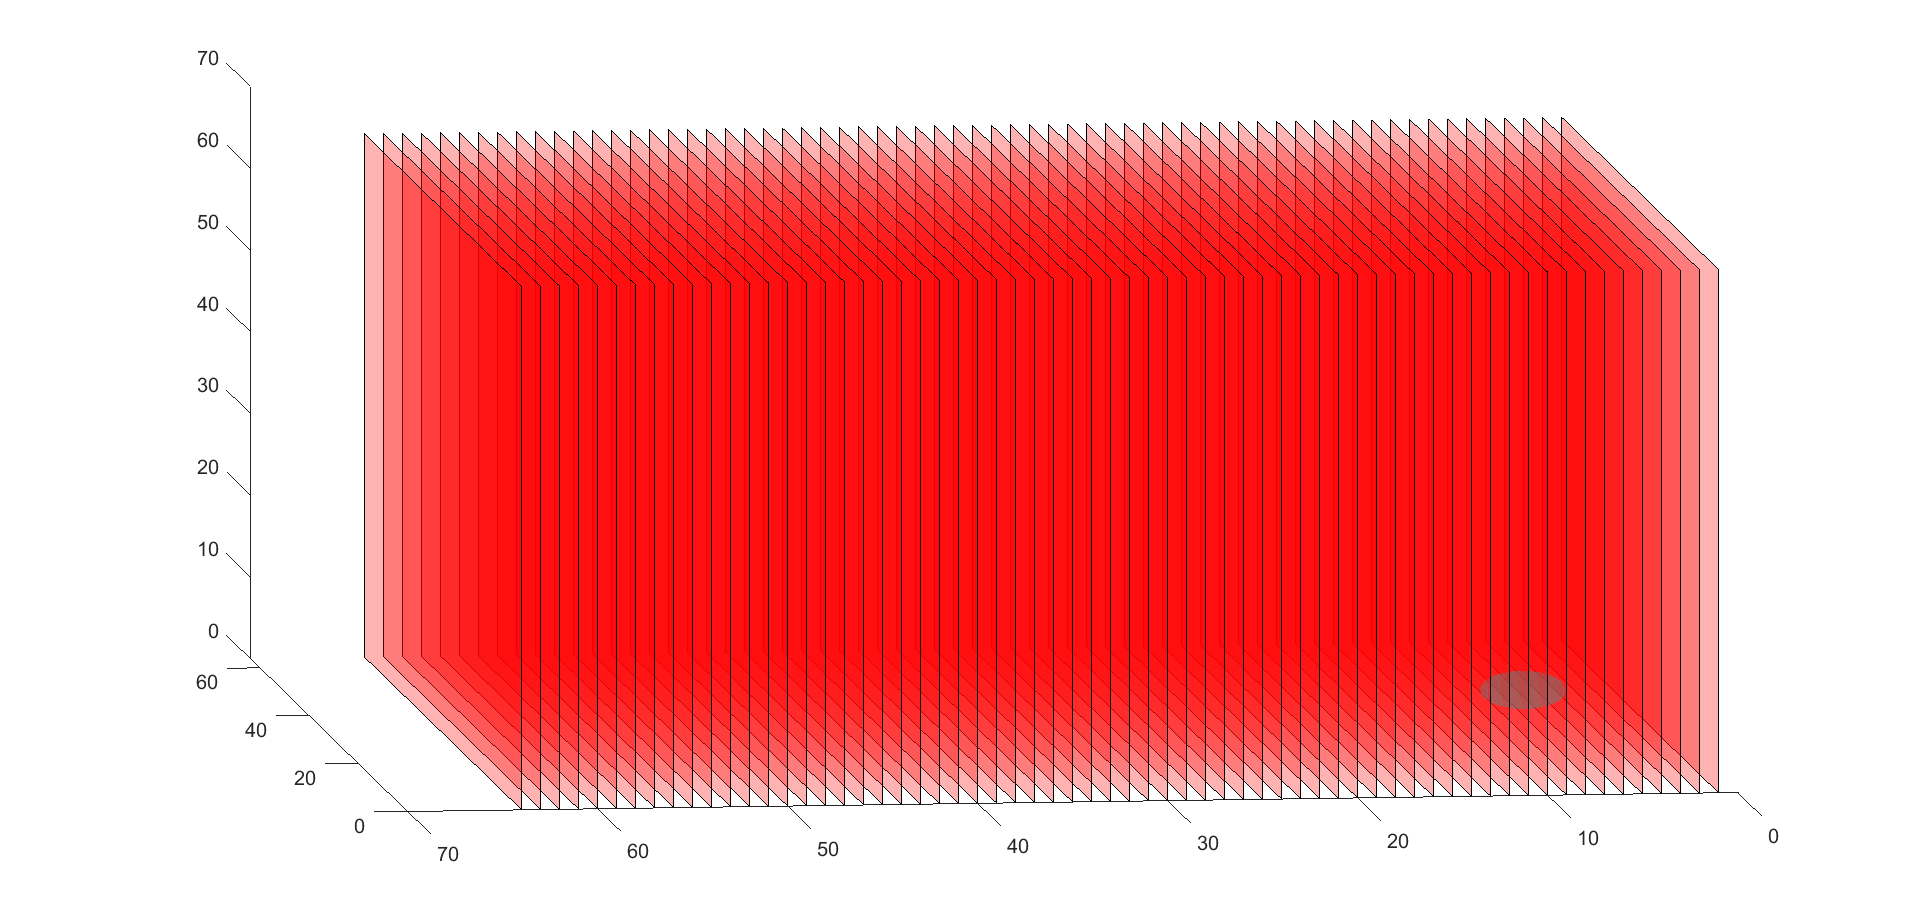
\includegraphics[scale=0.3]{./Figs/dataframes.png}
    \caption{Visualization of a dataset ($64$ x $64$ x $64$ 3D image). A marble is shown in the bottom left.}
  \label{fig:dviz}
\end{figure}

In order to reduce the noise content of the data, FFT approach is used. FFT allows us to transfer problem from time domain to the frequency domain and vice-versa. In frequency domain, the frequency associated with the marble (center frequency) can be obtained by averaging the spectrum, assuming the noise content is random (white noise). Once the center frequency is obtained, the noise in spectrum can be attenuated by using band-filters like Gaussian filter. Gaussian filter acts as a low-pass filter, in relation to the center frequency, that removes higher frequencies. This low-noise spectrum can then be tranformed back into the  time domain through inverse FFT to find the position of marble. \\
In Section \ref{Introduction}, more detailed theoretical background on Fourier transform, spectral averaging and filtering is discussed. Section \ref{Algorithm} outlines algorithms used as pseudocode and Section \ref{Result} contains computational results  of analysis the ultrasound data using FFT approach.

\pagebreak
%  Theoretical Background
\section{Theoretical Background}\label{Introduction}
Any function in the interval $x \in (-L, L]$, can be expressed in terms of linear combination of sinusoidal functions $A \cos(2 \pi fx + \phi)$ of different amplitudes (A), frequencies (f) and phases($\phi$), known as Fourier series. For functions with discontinuity in the interval, mean value can be used. 

\begin{equation}\label{eqn:fourierseries}
    f(x) = \frac{a_0}{2} + \sum_{i=1}^\infty \left(a_n\cos{\frac{n \pi}{L}x} + b_n\sin{\frac{n \pi}{L}x}\right) \quad x \in (-L,L].
\end{equation}
Using the orthoganility of $\cos(x)$ and $\sin(x)$ functions, we can find the coefficients as
\begin{align*}
a_0 &= \frac{1}{2L}\int_{-L}^{L} f(x) dx 
&a_n &= \frac{1}{L}\int_{-L}^{L} f(x) \cos{\frac{n \pi}{L}}x dx 
&b_n &= \frac{1}{L}\int_{-L}^{L} f(x) \sin{\frac{n \pi}{L}x}dx 
\end{align*}

Using exponential form of the $\cos(x) = \frac{e^{ix} + e^{-ix}}{2}$ and $\sin(x) = \frac{e^{ix} - e^{-ix}}{2i}$ in above equation, we can also express $f(x)$ in complex exponential form.
\begin{align*}
&f(x) = \sum_{-\infty}^{\infty} c_n e^{\frac{in \pi}{L}x}  \quad \in (-L,L]. 
&c_n = \frac{1}{2L}\int_{-L}^{L} f(x) e^{-\frac{in \pi}{L}x} dx
\end{align*}

Fourier tranform of any periodic function in the interval $x \in (-\pi, \pi]$ is a complex valued function of frequency whose modulus is the amount of that frequency and argument is the phase of the sinusoid. Fourier transform and its inverse are defined as
\begin{align*}
&F(k) = \frac{1}{\sqrt{2\pi}} \int_{-\infty}^{\infty} f(x)e^{-ikx} dx 
&f(x) = \frac{1}{\sqrt{2\pi}} \int_{-\infty}^{\infty} F(k)e^{ikx} dk
\end{align*}

While the equation might look mysterious, it is conceptually very intuitive. $e^{-ikx}$ rotates (winds) in clockwise direction about the origin in a unit circle on a complex plane with frequency $k$ (also known as winding frequency). Thus, the integrand $f(x)e^{-ikx}$ is the original function $f(x)$ rotating around the complex plane with frequency $k$ (like a coil around sphere). The integration of this integrand over all values of $x$ in the interval gives the center of mass of the function $f(x)e^{-ikx}$. The center of mass stays near $0$ for all values of frequencies, except when it is equal to the frequency of $f(x)$. When the winding frequency and the frequency of the function matches, the center of mass moves away from $0$ and the frequency signature of  function is detected. \\

Fast Fourier transform was the algorithm developed by Cooley and Tukey to quickly find the discrete Fourier tranform (DFT). Since there are $n$ multiplication and $n$ addition necessary, computing DFT directly requires $\mathcal{O}(n^2)$ operations. FFT uses the fact that odd and even sub-series can be computed concurrently. This forms a binary tree set of instructions that can be computed in $\mathcal{O}(n\log(n))$.
\begin{align*}
x[k] = \sum_{0}^{N-1} x[n] e^{-\frac{i\pi k[n]}{N}}  &=  \sum_{0}^{N/2-1} x[2n] e^{-\frac{i\pi k[2n]}{N}} + \sum_{0}^{N/2-1} x[2n+1] e^{-\frac{i\pi k[2n+1]}{N}} \\
&= \sum_{0}^{N/2-1} x[2n] e^{-\frac{i\pi k[n]}{N/2}} + e^{-ik \pi}\sum_{0}^{N/2-1} x[2n+1] e^{-\frac{i\pi k[n]}{N/2}}
\end{align*}

Since $x[-n] = x[n]^{*}$, the values for the negative frequencies can be simply appended at the end after finding complex conjugates. 

Spectral averaging is a technique to increase signal to noise ratio. Since FFT is a complex valued function, there are multiple ways one can average real and imaginary parts of complex numbers. Vector averaging involves averaging real and imaginary components separately. This is the method that has been implemented in this paper. Since, imaginary components arise due to the phase shift of the signal, averaging it separately could lead to random phase cancellation. Thus if one is using vector averaging, the signal in each data must be strictly in phase. This is equivalent to averaging in time-domain and it reduces the noise floor.
RMS averaging is another technique that preserves the energy of the spectrum. While it does not lower the noise floor, it decreases the noise fluctuation that helps to distinguish non-noise component.

Filtering the spectrum allows one to isolate signal from the noise. Gaussian filter is a simple low-pass band filter.
\[
G_f(k)=e^{-\tau (k - k_0)^2}
\]
where $\tau$ is the measure of the bandwidth and $k$ is the wave number.

% Algorithm Implementation and Development
\section{Algorithm Implementation and Development}\label{Algorithm}
The function implemented that estimates the path of the marble in the Fluff's intestine has four main components.
\begin{itemize}
\item Data acquisition and formatting: \\
Once the data is loaded, each instance is transformed into a 64 x 64 x 64 multidimensional array representing a 3D image. Spatial and spectral meshgrid is created over which input signal and spectrum assume their values respectively. Since FFT is defined over an interval $(-\pi, \pi]$, the wave number $k$ is scaled by $\pi /L$. $(-L, L]$ is the domain of input data with spatial resolution $\frac{2L}{N+1}$, where $N$ is the number of frequency modes chosen.
\item Spectral averaging: \\
Vector averaging of $20$ spectra obtained from MATLAB in-build FFT command \textit{fftn()} is performed to find the center frequency.
\item Gaussian filtering: \\
3D Gaussian filter  of unit bandwidth is implemented in frequency domain to isolate the center frequency from noise.
\item Path generation: \\
The filtered spectra are then inverse Fourier tranformed using MATLAB in-built command \textit{ifftn()}. The peak value for each signal data is calculated along with its coordinates. The coordinates are plotted to show the path traced by the marble.
\end{itemize}


\begin{algorithm}\label{alg:function}
\begin{algorithmic}
\STATE{Import data from \texttt{Testdata.mat}}
\STATE{Initialize average spectrum $U_{ave}$}
\FOR{$j = 1:20$}
 	\STATE{Extract measurement $j$th, $U_n$ from \texttt{Undata}}
	\STATE{$U_{ave} = U_{ave} + FFT(U_n)$ }
\ENDFOR
\STATE{Find the center frequencies $k_c$}
\STATE{Implement Gaussian filter, $G_f(k)$}
\STATE{Initialize path array}
\FOR{$j = 1:20$}
 	\STATE{Extract measurement $j$th from \texttt{Undata}}
	\STATE{FFT}
	\STATE{Filter the spectrum}
	\STATE{Inverse FFT}
	\STATE{Find peak value and location}
	\STATE{Append location to path}
\ENDFOR
\end{algorithmic}
\caption{Homework01.m}
\end{algorithm}

% Computational Results
\section{Computational Results}\label{Result}
The isosurface plot of vector averaged spectrum is shown in the Figure \ref{fig:ave}. The green blob represents the center frequency vector $k_c$. 
\[
k_c = [1.8850, -1.0472, 0]
\] 
Based on this frequency, Gaussian filter was designed to filter the noise in the spectrum. The Figure \ref{fig:iso} shows the isosurface plot of performing FFT, Gaussian filtering and inverse FFT operations on the $20$th dataset. The denoised spatial data clearly shows the location of the marble. The coordinates of marble at each instance of time were obtained by finding the indices associated with the peak value of the denoised data.The location at 20th instance was found to
\[
[x, y, z] = [-5.6250, 4.2188, -6.0938]
\] 
The Figure \ref{fig:path} shows the path of the marble for $20$ instances of time.

\begin{figure}[!b]
  \centering
    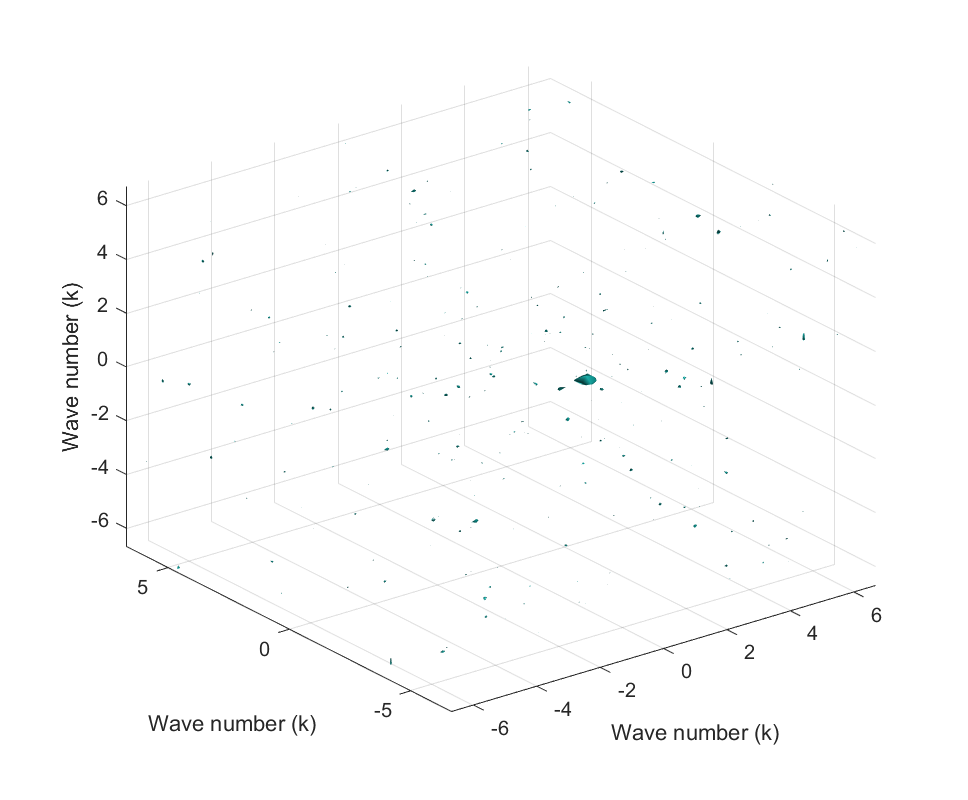
\includegraphics[scale=0.4]{./Figs/average_spectrum.png}
    \caption{Isosurface plot of the shifted and normalized average spectrum.}
  \label{fig:ave}
\end{figure}

% Summary and Conclusions
\section{Summary and Conclusions}
The center frequency was estimated after spectral averaging of $20$ spectra obtained from the FFT of raw datasets. Gaussian filter was implemented in frequency domain to isolate the center frequency from the noise. Denoised spatial data was then obtained by inverse FFT of the filtered spectrum. By finding the indices associated with the peak value of denoised data, marble's location was estimated. It was found that in order to break the marble, the laser must be pointed at the location $[-5.6250, 4.2188, -6.0938]$.

\begin{figure}[!t]
  \centering
    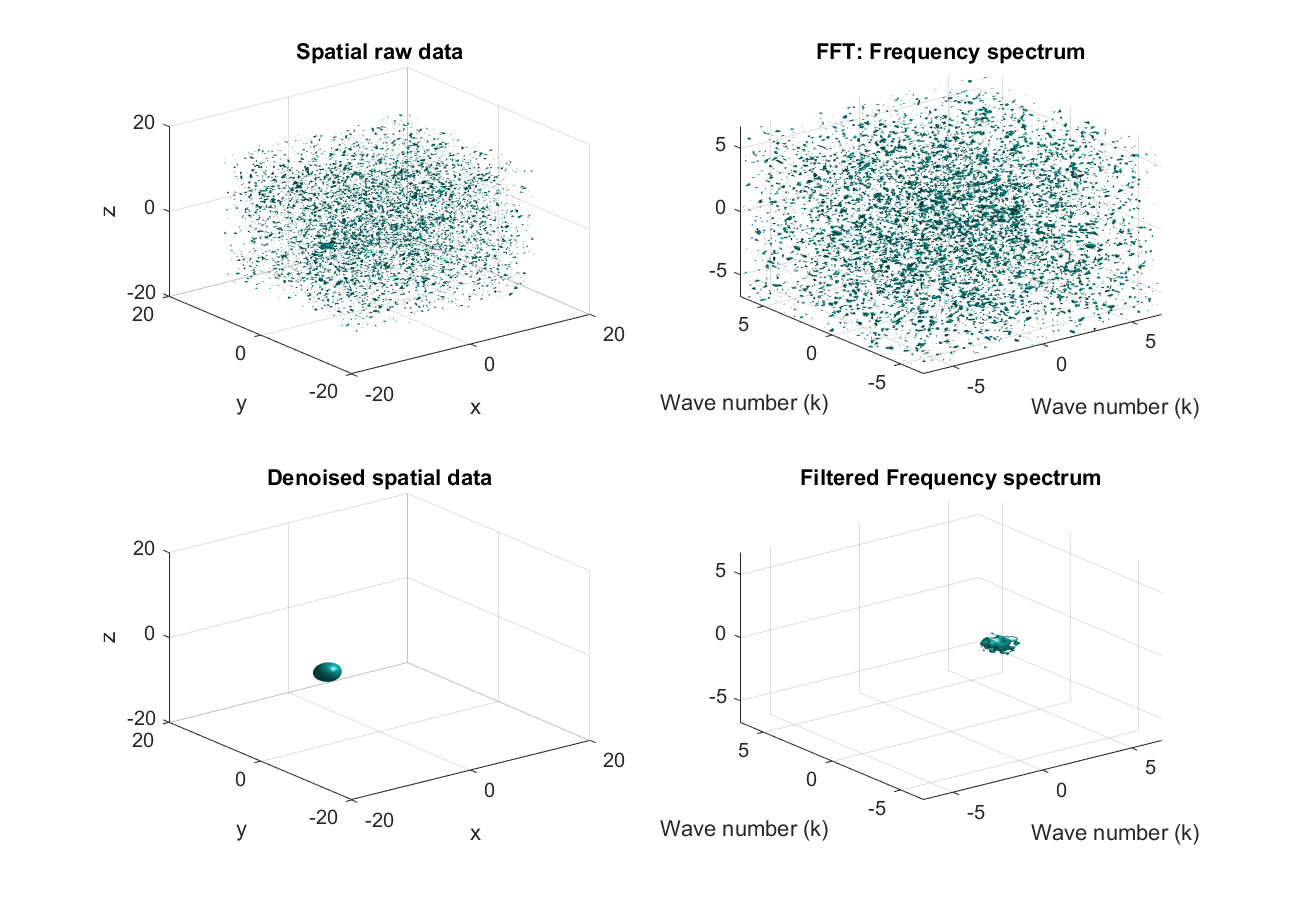
\includegraphics[width=\linewidth]{./Figs/isosurface.png}
    \caption{Figure shows isosurface plots of data at different stages of analysis. Raw spatial data (top left) is FFT to obtain frequency spectrum (top right). The frequency spectrum is then filtered using Gaussian filter to obtained filtered frequency spectrum (bottom right). And finally it is inverse FFT to obtain the denoised spatial data (botton left)}
  \label{fig:iso}
\end{figure}

\begin{figure}[!h]
  \centering
    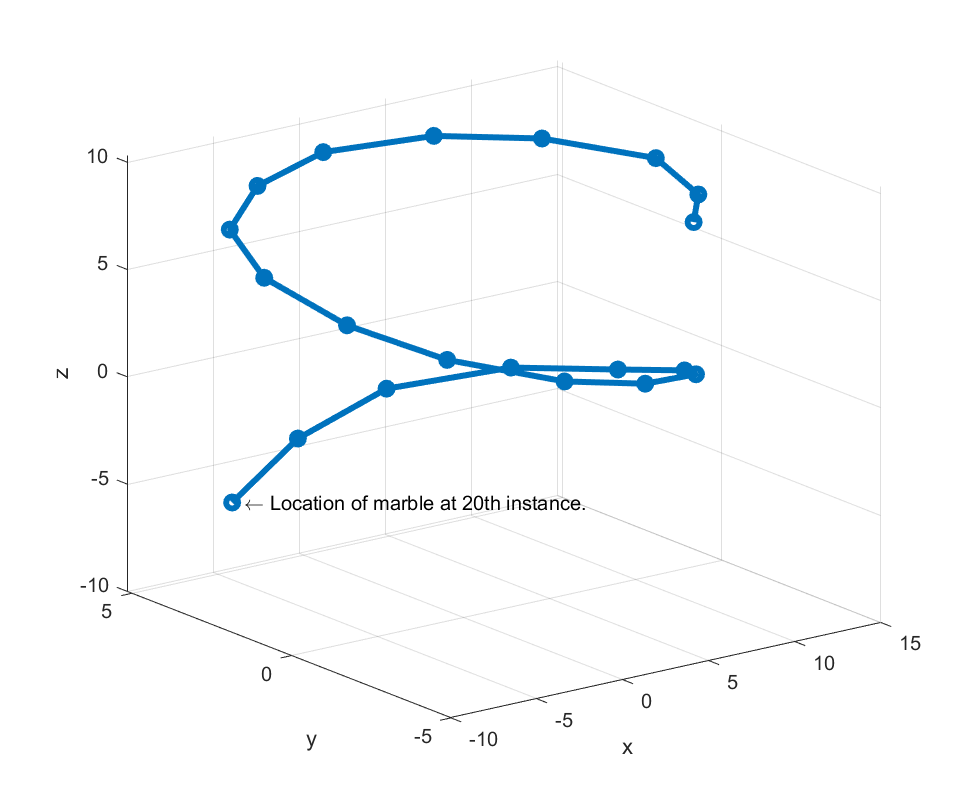
\includegraphics[scale=0.343]{./Figs/path.png}
    \caption{Path traced by the marble over $20$ instances of time.}
  \label{fig:path}
\end{figure}

\pagebreak
% Appendices
\begin{appendices}

% MATLAB Functions
\section{MATLAB Functions}
Some important MATLAB functions used during the implementation.
\begin{itemize}
    \item \texttt{y = linspace(x1,x2,n)} returns a row vector of \texttt{n} evenly spaced points between \texttt{x1} and \texttt{x2}. 
    \item \texttt{[X,Y,Z] = meshgrid(x,y,z)} returns 3-D grid coordinates defined by the vectors x, y, and z.
    \item \texttt{ks = fftshift(k)} rearranges FT by shifting zero frequency component to the center of the array. Exchanges two halves of the array.
    \item \texttt{Y = fftn(X)} returns multidimensional Fourier transform of an N-D array using FFT algorithm
    \item \texttt{Y = ifftn(X)} returns multidimensional discrete inverse Fourier transform of an N-D array using FFT algorithm
    \item \texttt{fv = isosurface(X,Y,Z,V,val} computes isosurface data from the volume data V at the isosurface value specified in val. Isosurface connects all points whose values at those points is val.
    \item \texttt{[row, col] = ind2sub(sz, ind)} returns the arrays row and col containing the equivalent row and column subscripts corresponding to the linear indices ind for a matrix of size sz.
    \item \texttt{B = reshape(A, sz)} reshapes A using  size vector sz.
    \item \texttt{fill3} function creates flat-shaded and Gouraud-shaded polygons.
\end{itemize}
A note to remember. When plotting isosurface plot (or any 3D plot) into subplot, you need to overwrite the view and lighting variables. When subplot is initialized, it assigns 2D plotting axes by default. \texttt{view(3)}; \texttt{camlight}; \texttt{lighting gouraud}

\pagebreak
% MATLAB Codes
\section{MATLAB Code}
\lstinputlisting[style=Matlab-editor]{Homework01.m}

%\begin{listing}[h]
%\inputminted{matlab}{example.m}
%\caption{Example code from external file.}
%\label{listing:examplecode}
%\end{listing}

\end{appendices}

\end{document}
